\chapter{IMPLEMENTATION}


% (20\% of Report Length)

% a. Showcase the output at various intermediate stages of the project pipeline

% b. Use proper data visualizing techniques to present the output

% c. Figures and tables must be accompanied by an explanation
\section{Tools Used}
\textbf{Figma}\\
Figma is a cloud-based design and prototyping tool that empowers teams to collaborate on UI/UX design projects in real-time. It offers a user-friendly interface and powerful features that make it a popular choice among designers. With Figma, designers can create and share interactive prototypes, design components, and design systems. Its cloud-based nature allows for seamless collaboration, enabling multiple team members to work on the same design simultaneously. Figma supports version control, ensuring that design iterations can be easily tracked and managed. \\
\textbf{React}\\
React is a widely-used open-source JavaScript library developed by Facebook for building user interfaces, particularly single-page applications where data changes frequently. It emphasizes a component-based architecture, allowing developers to create reusable UI components that encapsulate their own structure, logic, and styling. React’s use of a virtual DOM enhances performance by minimizing direct updates to the real DOM, ensuring efficient rendering. With its declarative approach, developers specify what the UI should look like based on different states, making the code more predictable and easier to debug. Additionally, React introduces JSX, a syntax extension that combines JavaScript and HTML, making it straightforward to write and understand UI components.\\
\textbf{Postgres}\\
PostgreSQL, often referred to simply as Postgres, is a powerful open-source relational database management system known for its reliability, robustness, and extensibility. Developed over decades and maintained by a global community of contributors, PostgreSQL offers a comprehensive set of features for managing structured data. It supports complex queries, transactions with ACID (Atomicity, Consistency, Isolation, Durability) properties, and a wide range of data types including JSON, XML, and spatial data. PostgreSQL's commitment to standards compliance and continuous improvement ensures compatibility with various programming languages and frameworks. With capabilities for scalability, data integrity, and advanced indexing, PostgreSQL is a preferred choice for applications requiring robust data management and high availability, contributing to its widespread adoption aweb industries from small startups to large enterprises. \\
\textbf{Git/Github}\\
Git is a distributed version control system that is both free and open-source, designed to handle projects of all sizes efficiently and swiftly. It simplifies collaboration by enabling multiple individuals to contribute changes that can be seamlessly merged into a single source. When using Git, the software runs locally on your computer, storing your files and their complete history. Alternatively, you can utilize online hosts like GitHub to store a copy of your files and their revision history. This central repository allows you to easily upload your changes and download updates from other developers, promoting seamless collaboration. Git facilitates automatic merging of changes, allowing multiple individuals to work on different sections of the same file and later merge their modifications without losing any work.\\
\textbf{Node Js with Express}\\
Node.js with Express.js is a powerful combination for building scalable and efficient web applications. Node.js provides a runtime environment that allows JavaScript to be executed server-side, leveraging its event-driven, non-blocking I/O model to handle multiple concurrent connections efficiently. Express.js, as a minimalist web framework for Node.js, simplifies the creation of APIs and routes, offering robust features such as middleware support, routing, and template engines. Together, Node.js and Express.js enable rapid development of RESTful APIs and web servers, making them well-suited for creating real-time applications, microservices, and backend systems. With a vibrant ecosystem of libraries and active community support, Node.js with Express.js remains a popular choice for developers seeking flexibility, performance, and scalability in web application development.\\
\textbf{JavaScript}\\
JavaScript is a programming language that is used to create interactive web pages and backend server. It is a powerful and versatile language that can be used to do a wide variety of things, including adding animation and interactivity to web pages, validating form data, processing user input, making Ajax requests to the server, and creating games and other interactive applications.\\
\textbf{Phaser}\\
Phaser is a powerful and popular open-source HTML5 game framework designed for creating 2D games that can run in both web browsers and mobile environments. Developed by Photon Storm, Phaser is known for its versatility and ease of use, making it a favorite among both beginner and experienced game developers. The framework supports Canvas and WebGL rendering, automatically selecting the best option based on the device's capabilities. Phaser offers a robust set of features including physics engines (Arcade Physics, P2 Physics, and Matter.js), input handling, asset management, animations, and audio integration. Its component-based architecture allows developers to build complex games by combining reusable pieces of code, enhancing modularity and maintainability. With an active community, extensive documentation, and numerous tutorials, Phaser provides ample resources for learning and development, empowering creators to bring their game ideas to life efficiently.
\section*{Postman}
Postman is a widely-used collaboration platform for API development, enabling developers to design, test, document, and monitor APIs with ease. Originally starting as a simple Chrome extension, Postman has evolved into a comprehensive tool that supports the entire API lifecycle. Its intuitive interface allows developers to construct and send HTTP requests to interact with APIs, receiving detailed responses to inspect and debug.

\section*{Unity 3D}
Unity 3D is a leading game development platform renowned for its ability to create both 2D and 3D interactive experiences across a wide range of platforms, including consoles, mobile devices, and VR/AR environments. Developed by Unity Technologies, the engine offers a comprehensive suite of tools that cater to every aspect of game development, from design and prototyping to final deployment.
Unity’s real-time rendering capabilities, coupled with its powerful physics engine, allow developers to create highly immersive and visually stunning games. The engine's support for WebGL enables developers to deploy their games directly to the web, providing browser-based experiences without the need for plugins. WebGL in Unity leverages the engine's advanced rendering capabilities, allowing developers to create complex 3D environments that run smoothly in any modern browser. This makes Unity a versatile tool not only for traditional game development but also for creating interactive web applications.


\subsection{Implementation Details of Modules}
This subsection outlines the implementation specifics for each module, detailing the core functionalities and algorithms utilized. It covers the programming languages, frameworks, and tools used in development, along with the interaction and communication between modules. Key design patterns, data management strategies, and error-handling mechanisms are discussed to ensure optimal performance. Additionally, security measures and optimizations applied during implementation are highlighted.
\newline
\newline
\textbf{Authentication Module}
\newline
The Authentication Module utilizes JSON Web Tokens (JWT) for secure user authentication. JWTs are compact, URL-safe tokens that encode user information, including a signature to verify the token's integrity. After a successful login, a JWT is generated and stored in an HTTP-only cookie, preventing unauthorized access via client-side scripts. The module also includes bcrypt hashing for securely storing user credentials and authentication middleware that checks the validity of the JWT on each request, ensuring only authenticated users can access protected resources.
\begin{figure}[H]
   \centering
    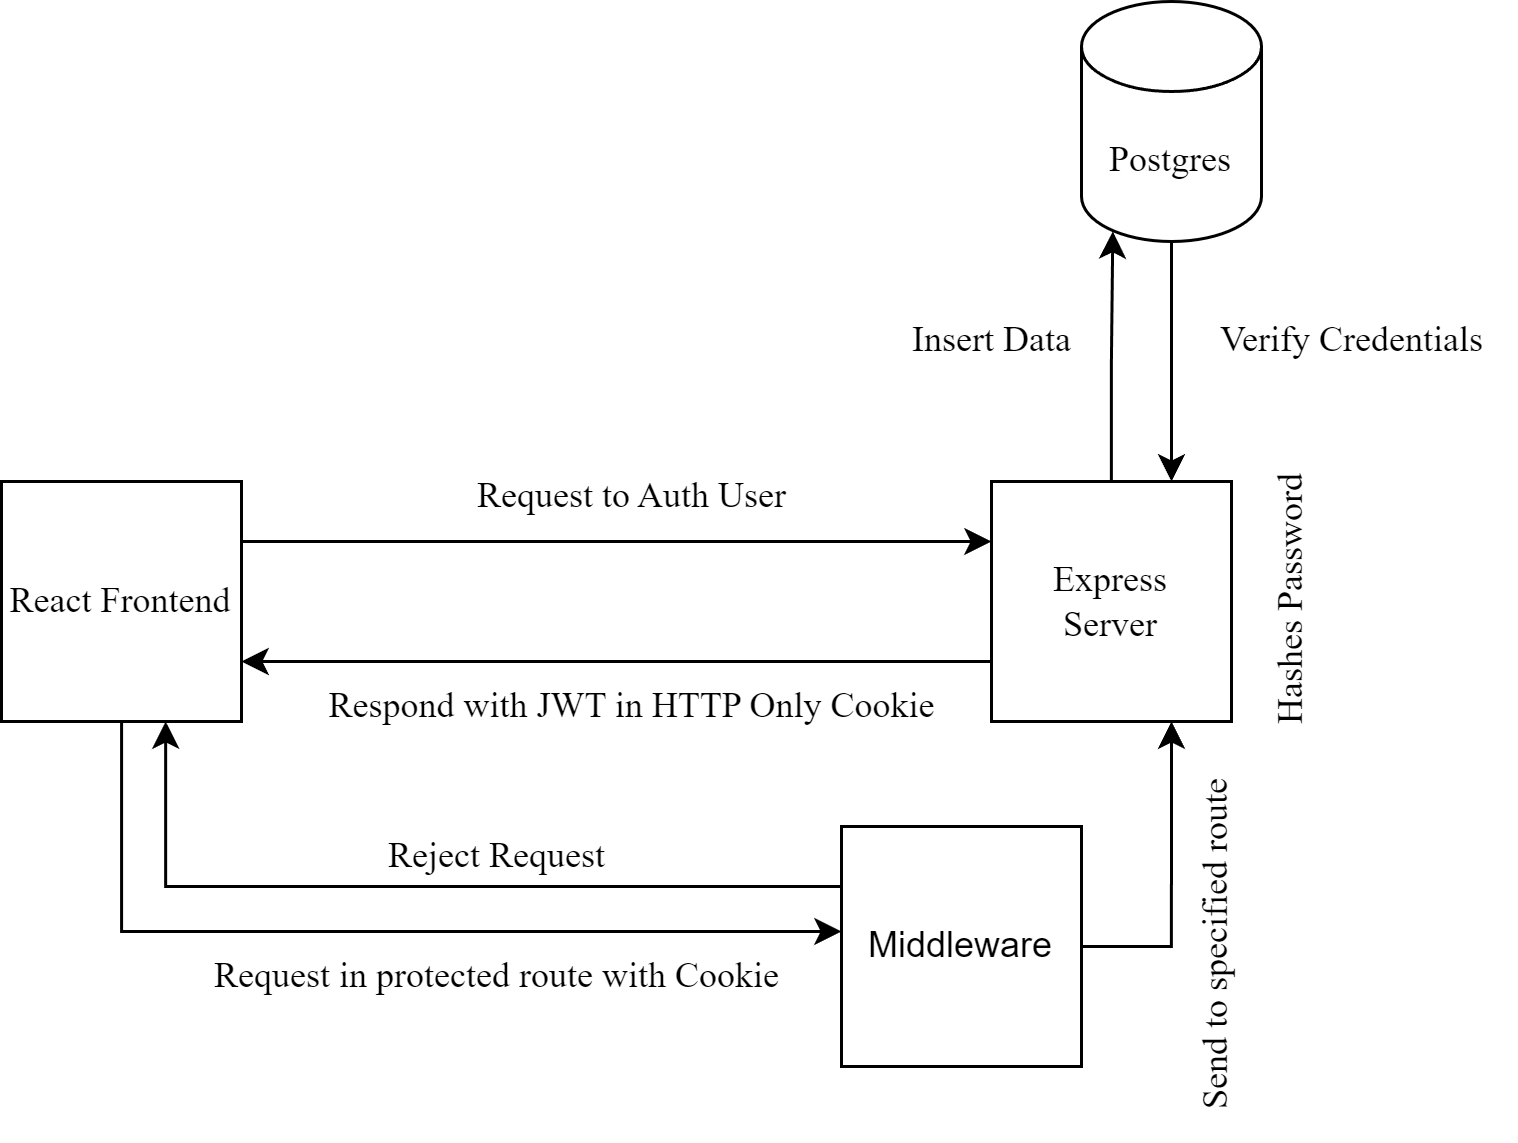
\includegraphics[height = 10cm]{Diagrams/auth module.png}
    \caption{Authnication Module}
\end{figure}
% \subsection{Algorithm Details}
% Here are some of the algorithms of our simulation models:

\subsection{Unit Testing Test Cases}
Theses API unit testing are performed using Postman. API unit testing using Postman involves creating and sending requests to API endpoints to ensure they function correctly. You can write test scripts in Postman to validate responses against expected outcomes, such as status codes and response content. Postman also allows for automating tests using the Collection Runner and Newman for continuous integration and delivery.
\begin{table}[H]
    \caption{Express Endpoint Testing: Capsules GET Methods}
    \label{tab:express_endpoint_testing}
    \resizebox{\textwidth}{!}{%
        \begin{tabular}{|p{0.5in}|p{2.5in}|p{3in}|p{1.5in}|}
            \hline
            \textbf{Test No.} & \textbf{Test Case} & \textbf{Endpoint} & \textbf{ Output} \\
            \hline
            1 & Getting Capsules By Category & \texttt{/api/capsule/category?category\newline=physics} & Returns JSON response with Array of Objects with specific category \\
            \hline
            2 & Getting Capsules By Id & \texttt{/api/capsule/?capsuleId=1} & Returns JSON response with Object of Capsules with specific id  \\
            \hline
            3 & Getting All Capsules & \texttt{/api/capsule/all} & Returns JSON response with Array of Objects of Capsules \\
            \hline
        \end{tabular}%
    }
\end{table}
\begin{table}[H]
    \caption{Express Endpoint Testing: Capsules GET Methods}
    \label{tab:express_endpoint_testing}
    \resizebox{\textwidth}{!}{%
        \begin{tabular}{|p{0.5in}|p{2.5in}|p{3in}|p{1.5in}|}
            \hline
            \textbf{Test No.} & \textbf{Test Case} & \textbf{Endpoint} & \textbf{ Output} \\
            \hline
            1 & Login user/admin endpoint & \texttt{/api/user/login\newline body: Username and Password} & Creates JWT token and sets an HTTP Only Cookie to the client side \\
            \hline
            2 & api/user/register & \texttt{/api/capsule/category?category\newline=physics} & Returns JSON response with Array of Objects with id \\
            \hline
           
        \end{tabular}%
    }
\end{table}
\begin{table}[H]
    \caption{Express Endpoint Testing: User Methods}
    \label{tab:express_endpoint_testing}
    \resizebox{\textwidth}{!}{%
        \begin{tabular}{|p{0.5in}|p{2.5in}|p{3in}|p{1.5in}|}
            \hline
            \textbf{Test No.} & \textbf{Test Case} & \textbf{Endpoint} & \textbf{ Output} \\
            \hline
            1 & Admin add capsule endpoint & \texttt{api/admin/add\newline body:capsule informations and images} & Sucessfully adds images in uploads folder and corresponding capsule into database  \\
            \hline
            
        \end{tabular}%
    }
\end{table}
\newpage
\subsection{Test Cases for System Testing}
System Testing involves a comprehensive evaluation of the entire PERN application, including both frontend and backend components. This phase aims to validate that all integrated parts of the system function correctly and cohesively. We will test the complete application flow to ensure seamless interaction between the frontend and backend, as well as to verify that the application meets its specified requirements and performs as expected.
\begin{table}[H]
    \caption{System/Application Testing: Capsules GET Methods}
    \label{tab:express_endpoint_testing}
    \resizebox{\textwidth}{!}{%
        \begin{tabular}{|p{0.5in}|p{2.5in}|p{3in}|p{1.5in}|}
            \hline
            \textbf{Test No.} & \textbf{Test Case} & \textbf{Input} & \textbf{ Output} \\
            \hline
            1 & Acessing Specific Capsules By Id & \texttt{/capsule/8\newline} & Shows whole capsule its images, pdf and all its meta information with quiz \\
            \hline
            2 & Acessing Capsules Menu By Category & \texttt{/capsules/physics} & Shows cards, thumbnail, title, description and buttons about related category capsules  \\
            \hline
            3 & Getting All Capsules & \texttt{/learning-area} & Shows Learning Capsules with categories of each capsules \\
            \hline
        \end{tabular}%
    }
\end{table}
\begin{table}[H]
    \caption{System/Application Testing: Login}
    \label{tab:express_endpoint_testing}
    \resizebox{\textwidth}{!}{%
        \begin{tabular}{|p{0.5in}|p{2.5in}|p{3in}|p{1.5in}|}
            \hline
            \textbf{Test No.} & \textbf{Test Case} & \textbf{Input} & \textbf{ Output} \\
            \hline
            1 & Login User & \texttt{/login\newline Input: Username 'test' and Password 'test'} & Creates JWT token and sets an HTTP Only Cookie to the client side and redirects user into profile page\\
            \hline
            1 & Login Admin & \texttt{/login\newline Input: Username 'Admin' and Password 'admin'} & Creates JWT token and sets an HTTP Only Cookie to the client side and redirects user into profile page also shows Admin Button for Admin Panel\\
            \hline
           
        \end{tabular}%
    }
\end{table}
\begin{table}[H]
    \caption{System/Application Testing: User Methods}
    \label{tab:express_endpoint_testing}
    \resizebox{\textwidth}{!}{%
        \begin{tabular}{|p{0.5in}|p{2.5in}|p{3in}|p{1.5in}|}
            \hline
            \textbf{Test No.} & \textbf{Test Case} & \textbf{Input} & \textbf{ Output} \\
            \hline
            1 & Admin add capsule & \texttt{/admin/add} & Shows Form to add capsules and adds capsules when submitted  \\
            \hline
            
        \end{tabular}%
    }
\end{table}